\documentclass[a4paper, 12pt]{article}%тип документа

%отступы
\usepackage[left=2cm,right=2cm,top=2cm,bottom=3cm,bindingoffset=0cm]{geometry}
\setlength{\parindent}{5ex}

%Русский язык
\usepackage[T2A]{fontenc} %кодировка
\usepackage[utf8]{inputenc} %кодировка исходного кода
\usepackage[english,russian]{babel} %локализация и переносы

%Вставка картинок
\usepackage{graphicx}
\graphicspath{{pictures/}}
\DeclareGraphicsExtensions{.pdf,.png,.jpg}

%Графики
\usepackage{pgfplots}
\pgfplotsset{compat=1.9}

%Математика
\usepackage{amsmath, amsfonts, amssymb, amsthm, mathtools}

%Таблицы
\usepackage{longtable} 
\usepackage{float}

%Римские цифры
\newcommand{\RomanNumeralCaps}[1]{\uppercase\expandafter{\romannumeral#1}}

\usepackage{multirow}


\begin{document}
	\begin{titlepage}
		\begin{center}
			\textsc{Федеральное государственное автономное образовательное учреждение высшего образования«Московский физико-технический институт (национальный исследовательский университет)»\\[5mm]
			}
			
			\vfill
			
			\textbf{Отчёт по лабораторной работы 3.3.5\\[3mm]
				Эффект Холла
				\\[50mm]
			}
			
		\end{center}
		
		\hfill
		\begin{minipage}{.5\textwidth}
			Выполнил студент:\\[2mm]
			Сериков Василий Романович\\[2mm]
			группа: Б03-102\\[5mm]
			
		\end{minipage}
		\vfill
		\begin{center}
			Москва, 2022 г.
		\end{center}
		
	\end{titlepage}
	
	\newpage
	\textbf{Аннотация}\\
	
	
	\textbf{Цель работы: }\\
	Измерение подвижности и концентрации носителей заряда
	в металлах.\\
	
	\textbf{В работе используются: }\\
	Электромагнит с источником питания, источник постоянного тока, микровольтметр, амперметры, милливеберметр или
	цифровой магнитометр, образцы из меди, серебра и цинка.\\
	
	\textbf{Теоретические сведения: } \\
	В работе изучаются особенности проводимости металлов в геометрии
	мостика Холла. Ток пропускается по плоской прямоугольной металлической пластинке, помещённой в перпендикулярное пластинке магнитное
	поле. Измеряется разность потенциалов между краями пластинки в поперечном к току направлении. По измерениям определяется константа
	Холла, тип проводимости (электронный или дырочный) и на основе соотношения (3.28) вычисляется концентрация основных носителей заряда.
	
	Во внешнем магнитном поле B на заряды действует сила Лоренца:
	$$F = qE + qU \times B $$
	Эта сила вызывает движение носителей, направление которого в общем
	случае не совпадает с E. Действительно, траектории частиц будут либо искривляться, либо, если геометрия проводника этого не позволяет, возникнет дополнительное электрическое поле, компенсирующее магнитную составляющую силы Лоренца. Возникновение поперечного току электрического поля в образце, помещённом во внешнее магнитное поле, называют эффектом Холла.
	
	Мостик Холла. В данной схеме ток вынуждают течь по оси x вдоль плоской пластинки (ширина пластинки a, толщина h, длина l). Сила Лоренца, действующая со стороны перпендикулярного пластинке магнитного поля, «прибивает» носители заряда к краям образца, что создаёт холловское электрическое поле, компенсирующее эту
	силу. Поперечное напряжение между краями пластинки (холловское напряжение) равно $U_\perp = E_ya $, где:
	$$ E_y = \rho_{yx} \cdot \jmath_x = \jmath_x B/nq $$
	Плотность тока, текущего через образец, равна $\jmath_x = I/ah$, где I — полный ток, ah — поперечное сечение. Таким образом, для холловского напряжения имеем
	$$U_\perp = B nqh I = RH Bh I $$
	где константу $RH = 1/nq$
	называют постоянной Холла. Знак постоянной Холла определяется
	знаком заряда носителей.\\
	
	\textbf{Экспериментальная установка: }\\
	В зазоре электромагнита создается постоянное магнитное поле, которое можно регулировать с помощью источника питания электромагнита.\\
	Иногда контакты 2 и 4 вследствие неточности подпайки не лежат на одной эквипотенциали, и тогда напряжение между ними связано не только с эффектом Холла, но и с омическим напряжением, вызванным протеканием основного тока через образец. \\
	Неточности измерений можно избежать путем фиксирования этого омического напряжения при нулевом значении силы тока и отсчитывании от него Холловского напряжения. 
	\[U_\perp = U_{24} - U_0\]
	Измерив ток в образце и напряжение $U_{34}$ между контактами 3 и 4 в отсутствии магнитного поля, можно, зная параметры образца, рассчитать проводимость материала образца по формуле:
	\begin{equation}
		\sigma = \dfrac{I L_{34}}{U_{34}al}
	\end{equation}
	\begin{figure}[H]
		\center{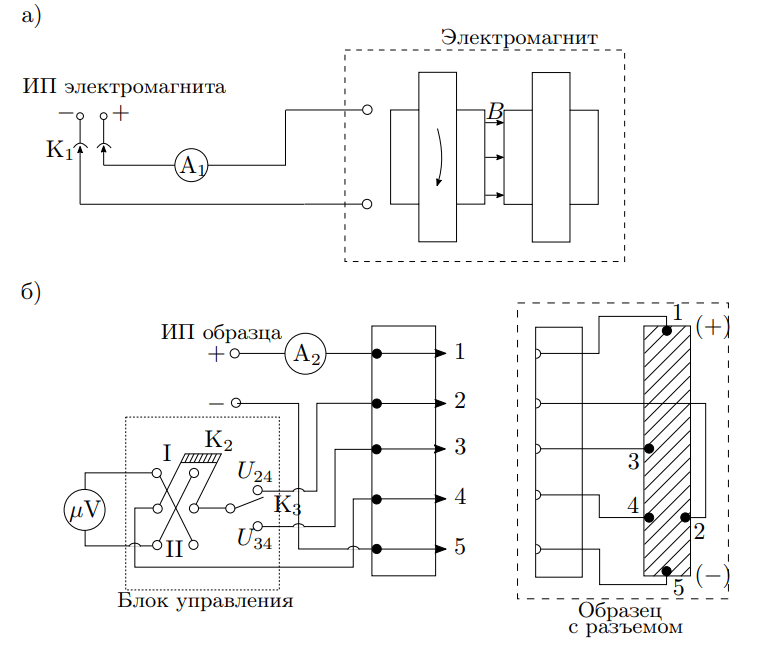
\includegraphics[scale=1]{ust.png}}
		\caption{Экспериментальная установка.}
	\end{figure}
	
	
	\newpage
	
	\textbf{Результаты измерений и обработка данных: }\\
	
	\textit{Градуировка электромагнита}
	\begin{enumerate}
		
	\item Измерим калибровочную кривую электромагнита — зависимость
	между индукцией B магнитного поля в его зазоре и током $I_M$ через обмотки магнита. Полученные данные занесем в таблицу 1 и построим по ним график зависимости $B(I_M)$. 
		
	\begin{longtable} {|c|c|c|c|c|c|c|c|c|c|c|c|}
		\hline
		$I_M$, A& 0 & 0,1 & 0,2 & 0,3 & 0,4 & 0,5 & 0,6 & 0,7 & 0,8 & 1,0 & 1,2  \\ \hline
		$B$, мТл & 18,7 & 150,2 & 276,8 & 386,3 & 540,0 & 614,5 & 751,8 & 900,0 & 1031,7 & 1153,6 & 1220,0 \\ \hline
		\caption{Данные для калибровочной кривой магнита}
	\end{longtable}
		
	\begin{figure}[H]
		\center{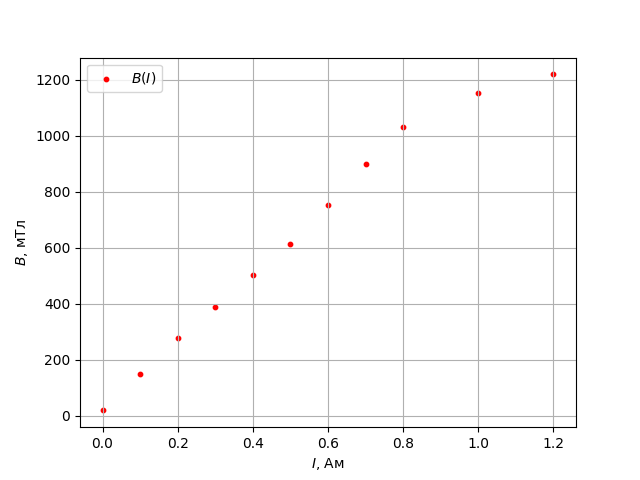
\includegraphics[scale=1]{B(I).png}}
		\caption{График зависимости B(I) для калибровочной кривой электромагнита.}
	\end{figure}

	\textit{Измерение ЭДС Холла}\\
	
	\item Получим зависимость напряжения $U_{24}$ от тока электромагнита $I_M$ при фиксированном
	токе I через образец меди, аналогично получим зависимость при других значениях тока I через образец. Аналогично для образца из цинка при одном значении тока I = 1 Ам Полученные данные занесем в таблицы 2-8.$\sigma_U = 1 \text{ дел} = 40$ нВ
	
	\begin{longtable} {|c|c|c|c|c|c|c|c|}
		\hline
		$I_M$, A & 0,1 & 0,19 & 0,39 & 0,6 & 0,8 & 1,0 & 1,2  \\ \hline
		$U$, дел & 4 & 5 & 6 & 7 & 8,5 & 9 & 10 \\ \hline
		\caption{Зависимость $U(I_M)$ для меди при I = 0,21 А, $U_0$ = 2 дел}
	\end{longtable}
	
		
	\begin{longtable} {|c|c|c|c|c|c|c|c|c|c|}
		\hline
		$I_M$, A & 0,1 & 0,2 & 0,3 & 0,4 & 0,5 & 0,6 & 0,7 & 0,9 & 1,1  \\ \hline
		$U$, дел & 5 & 6 & 8 & 9 & 10,5 & 13 & 14 & 16 & 17 \\ \hline
		\caption{Зависимость $U(I_M)$ для меди при I = 0,4 А, $U_0$ = 3 дел}
	\end{longtable}

	\begin{longtable} {|c|c|c|c|c|c|c|c|c|c|}
		\hline
		$I_M$, A & 0,1 & 0,2 & 0,3 & 0,4 & 0,5 & 0,6 & 0,7 & 0,9 & 1,1  \\ \hline
		$U$, дел & 6 & 8 & 10,5 & 12,5 & 15 & 17 & 19 & 22 & 23 \\ \hline
		\caption{Зависимость $U(I_M)$ для меди при I = 0,6 А, $U_0$ = 4 дел}
	\end{longtable}
		
	\begin{longtable} {|c|c|c|c|c|c|c|c|c|c|}
		\hline
		$I_M$, A & 0,1 & 0,2 & 0,3 & 0,4 & 0,5 & 0,6 & 0,7 & 0,9 & 1,1  \\ \hline
		$U$, дел & 7 & 9,5 & 12,5 & 15,5 & 18 & 21 & 23 & 27 & 29 \\ \hline
		\caption{Зависимость $U(I_M)$ для меди при I = 0,8 А, $U_0$ = 4 дел}
	\end{longtable}
		
	\begin{longtable} {|c|c|c|c|c|c|c|c|c|c|}
		\hline
		$I_M$, A & 0,1 & 0,2 & 0,3 & 0,4 & 0,5 & 0,6 & 0,7 & 0,9 & 1,1  \\ \hline
		$U$, дел & 7 & 11 & 15 & 18 & 22 & 25 & 28 & 32,5 & 35 \\ \hline
		\caption{Зависимость $U(I_M)$ для меди при I = 1 А, $U_0$ = 4 дел}
	\end{longtable}
		
	
	\begin{longtable} {|c|c|c|c|c|c|c|c|c|c|}
		\hline
		$I_M$, A & 0,1 & 0,2 & 0,3 & 0,4 & 0,5 & 0,6 & 0,7 & 0,9 & 1,1  \\ \hline
		$U$, дел & 8 & 13 & 17,5 & 21,5 & 26 & 30 & 33 & 39 & 42,5 \\ \hline
		\caption{Зависимость $U(I_M)$ для меди при I = 1,2 А, $U_0$ = 4 дел}
	\end{longtable}
		
	\begin{longtable} {|c|c|c|c|c|c|c|c|c|c|c|c|c|}
		\hline
		$I_M$, A & 0,1 & 0,2 & 0,3 & 0,4 & 0,5 & 0,6 & 0,7 & 0,8 & 0,9 & 1,0 & 1,1 & 1,2  \\ \hline
		$U$, дел & 18,5 & 14,5 & 10 & 6 & 3,5 & 0 & -3 & -6 & -7,5 & -9 & -10,5 & -11,5 \\ \hline
		\caption{Зависимость $U(I_M)$ для цинка при I = 1 А, $U_0$ = 23 дел}
	\end{longtable}
		
	
	\newpage
	\textit{Определение удельной проводимости}\\
	
	\item При токе $I = 1 $ А через образец измерим падение напряжения между контактами 3 и 4 для каждого из двух образцов.\\
	для цинка: $U = 310 \pm 5$ мкВ, $L_{3,4} = 3,5$ мм, a = 0,12 мм, l = 9 мм\\
	для меди: $U = 470 \pm 5$ мкВ, $L_{3,4} = 6$ мм, a = 0,05 мм, l = 8 мм\\
	
	\item Построим графики зависимости $U(B)$ для полученных значений. По коэффициентам полученных прямых построим график зависимости $k(I)$ для меди.
	
	
	\begin{figure}[H]
		\center{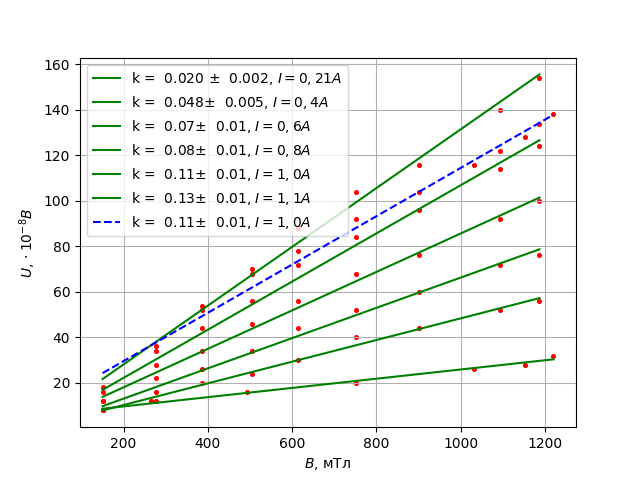
\includegraphics[scale=1]{U(B).png}}
		\caption{График зависимости U(B) для меди (сплошная) и цинка (пунктир).}
	\end{figure}

	\begin{figure}[H]
		\center{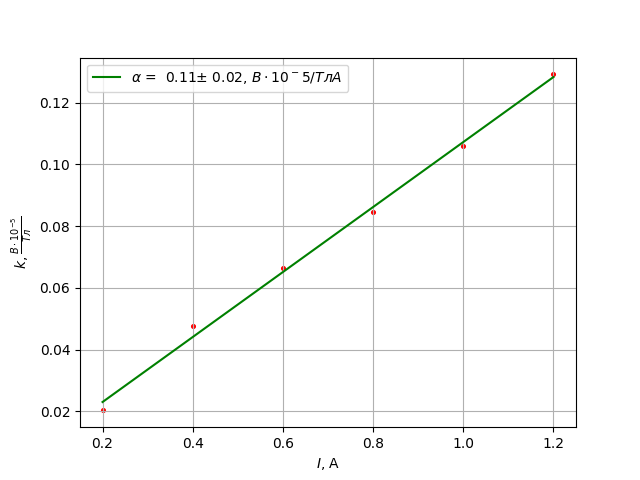
\includegraphics[scale=1]{k(I)Cu.png}}
		\caption{График зависимости k(I) для меди.}
	\end{figure}
		
	\item Для обоих образцов рассчитаем постоянную Холла $R_H$, концентрацию n носителей тока,
	удельное сопротивление $\rho_{\text{уд}}$ и удельную проводимость $\sigma_0$ материалов.\\
	
	\textit{Медь:}\\
	$$ R_H = - \alpha \cdot a = - (5,5 \pm 0,5 \cdot 10^{-11}) \text{м}^3/\text{Кл}$$
	
	$$ n = \frac{1}{R_H e} = (1,3 \pm 0,3 \cdot 10^{29}) 1/\text{м}^3$$
	
	$$ \sigma_0 = \frac{IL_{34}}{al U} = (0,32 \pm 0,06 \cdot 10^8) 1/\text{Ом м} $$	
	\textit{Цинк:}\\
	$$ R_H = k \cdot a/I = (12 \pm 1 \cdot 10^{-11}) \text{м}^3/\text{Кл}$$
	
	$$ n = \frac{1}{R_H e} = (0,5 \pm 0,1 \cdot 10^{29}) 1/\text{м}^3$$
	
	$$ \sigma_0 = \frac{IL_{34}}{al U} = (0,11 \pm 0,02 \cdot 10^8) 1/\text{Ом м} $$	
	
	\item . Используя найденные значения концентрации n и удельной проводимости $\sigma_0 = 1/\rho$ вычислим подвижность $\mu$ носителей тока. Сведем все результаты в таблицу.
	
	\begin{longtable} {|c|c|c|c|c|c|}
		\hline
		Металл & $R_H$, $\text{м}^3/\text{Кл}$  & Табл. $R_H$, $\text{м}^3/\text{Кл}$ &  n, $1/\text{м}^3$ & $\sigma$, $1/\text{Ом м}$& b, $\text{см}^2/Bc$ \\ \hline
		Медь & $- 5,5 \pm 0,5 \cdot 10^{-11}$ &$ - 5,5 \cdot 10^{-11}$ & $1,3 \pm 0,3 \cdot 10^{29}$ & $0,32 \pm 0,06 \cdot 10^8$ &$17 \pm 1$   \\ \hline
		Цинк & $ 12 \pm 1 \cdot 10^{-11}$ & $10\cdot 10^{-11}$ & $ 0,5 \pm 0,1 \cdot 10^{29} $ & $0,11 \pm 0,02 \cdot 10^8$ &$ 13 \pm 1$ \\ \hline
		\caption{Сводная таблица всех полученных результатов}
	\end{longtable}
		
	\end{enumerate}
	
	\textbf{Обсуждение результатов и выводы: }\\
	
	В данной работе мы изучали эффект Холла и измерили подвижность, концентрацию и постоянную Холла для образцов меди и цинка.
	Полученные нами постоянные Холла близки к табличным значениям, однако удельные проводимости не совпадают ($0,56 \cdot 10^8 \dfrac{1}{\text{Ом} \cdot \text{м}}$ для меди и $0,16 \cdot 10^8 \dfrac{1}{\text{Ом} \cdot \text{м}}$ для цинка), есть предположение, что мы не правильно сняли значения напряжения между контактами 3 и 4, что стало причиной такого отклонения от табличного значения.
	
	
	
	
	
	
	
	
	
	
	
	
	
	
	
	
	
	
	
	
	
	
	
	
	
	
	
	\end{document}